% Generation and refinement of 2D triangular meshes
% by Patrick Meury

\chapter{Mesh Generation and Refinement} \label{chap:mesh_gen} \index{mesh|(}

This chapter contains the documentation for the \MATLAB library \LIBNAME of the mesh data structures and the mesh
generation/refinement routines. Currently the library supports creation of 2D structured triangular meshes for nearly
arbitrarily shaped domains. Furthermore it is possible to create unstructured quadrilateral meshes by a kind of morphing
procedure from triangular meshes. Structured meshes for both triangular and quadrilateral elements can be obtained throu
uniform red refinements from coarse initial meshes.

\section{Mesh Data Structure} \label{sect:mesh_data} \index{mesh!data structure} \index{mesh@{\tt Mesh}|textit}
\label{sect:MDS}

All meshes in \LIBNAME are represented as \MATLAB structs. This makes it possible to encapsulate all data of a mesh
inside only one variable in the workspace.

For the rest of this manual we denote by $M$ the number of vertices, by $N$ the number of elements and by $P$ the
number of edges for a given mesh.

The basic description of mesh contains the fields {\tt Coordinates} of vertex coordinates, and a list of elements
connecting them, corresponding to the field {\tt Elements}. The details of this data structure can be seen on table
\ref{tab:MSH_B}.

\begin{table}[htb]
  \begin{tabular}{p{2cm}p{9cm}}
    \ttitindex{Coordinates} & {\small $M$-by-$2$ matrix specifying all vertex coordinates} \\
    \ttitindex{Elements} & {\small $N$-by-$3$ or $N$-by-$4$ matrix connecting vertices into elements}
  \end{tabular}
  \caption{Basic mesh data structure}
  \label{tab:MSH_B}
\end{table}


When using higher order finite elements we need to place global degrees of freedom on edges of the mesh. Even though a mesh is fully determined by the fields {\tt Coordinates} and {\tt Elements} it is necessary to extend the basic mesh data structure by edges and additional connectivity tables connecting them to
elements and vertices. A call to the following routine \\

\noindent{\tt >> Mesh = \ttitindex{add\_Edges}(Mesh);} \\

\noindent will append the fields {\tt Edges} and {\tt Vert2Edges} to any basic mesh data structure containing the fields
{\tt Coordinates} and {\tt Elements}. Detailed information on the additional fields can be found on table \ref{tab:MSH_E}.

\begin{table}[htb]
  \begin{tabular}{p{2cm}p{9cm}}
    {\tt Coordinates} & {\small $M$-by-$2$ matrix specifying all vertex coordinates}                 \\
    {\tt Elements}    & {\small $N$-by-$3$ or $N$-by-$4$ matrix connecting vertices into elements}   \\
    \ttitindex{Edges} & {\small $P$-by-$2$ matrix specifying all edges of the mesh} \\
    \ttitindex{Vert2Edge}   & {\small $M$-by-$M$ sparse matrix specifying the edge number
                        of the edge connecting vertices {\tt i} and {\tt j} (or zero
                        if there is no edge)}
  \end{tabular}
  \caption{Mesh with additional edge data structure}
  \label{tab:MSH_E}
\end{table}

To be able to incorporate boundary conditions into our variational formulations we need to seperate boundary edges
from interior edges. Calling the function \\

\noindent {\tt >> Loc = \ttitindex{get\_BdEdges}(Mesh);} \\

\noindent provides us with a locator {\tt Loc} of all boundary edges of the mesh in the field {\tt Edges}. For all the boundary edges flags that specify the type of the boundary condition can be set. They are written in the field {\tt BdFlags} and the convention is that every boundary edge gets a negative flag while the edges in the interior are flaged by 0.

When using discontinuous Galerkin finite element methods or edge-based adaptive estimators we need to compute jumps
of solutions across edges. This makes it necessary to be able to determine the left and right hand side neighbouring
elements of each edge. The function call \\

\noindent {\tt >> Mesh = \ttitindex{add\_Edge2Elem}(Mesh);} \\

\noindent adds the additional field {\tt Edge2Elem}, which connects edges to their neighbouring elements for any mesh
data structure containing the fields {\tt Coordinates}, {\tt Elements}, {\tt Edges} and {\tt Vert2Edge}. For details
consider table \ref{tab:MSH_E2}.

\begin{table}[htb]
  \begin{tabular}{p{2cm}p{9cm}}
    {\tt Coordinates} & {\small $M$-by-$2$ matrix specifying all vertex coordinates}                \\
    {\tt Elements}    & {\small $N$-by-$3$ or $N$-by-$4$ matrix connecting vertices into elements}  \\
    {\tt Edges}       & {\small $P$-by-$2$ matrix specifying all edges of the mesh}                 \\
    {\tt Vert2Edge}   & {\small $M$-by-$M$ sparse matrix specifying the edge number
                        of the edge connecting vertices {\tt i} and {\tt j} (or zero
                        if there is no edge)}                                                       \\
    \ttitindex{Edge2Elem}   & {\small $P$-by-$2$ matrix connecting edges to their neighbouring
                        elements. The left hand side neighbour of edge {\tt i} is given
                        by {\tt Edge2Elem(i,1)}, whereas {\tt Edge2Elem(i,2)} specifies
                        the right hand side neighbour, for boundary edges one entry is $0$}		\\
    \ttitindex{EdgeLoc}	&	{\small $P$-by-$3$ or $P$-by-$4$ matrix connecting egdes to local edges of elements.}
  \end{tabular}
  \caption{Mesh with additional edge data structure and connectivity table}
  \label{tab:MSH_E2}
\end{table}

In some finite element applications we need to compute all sets of elements sharing a specific vertex of the mesh.
These sets of elements, usually called patches, can be appended to any mesh containing the fields {\tt Coordinates}
and {\tt Elements} by the following routine \\

\noindent {\tt >> Mesh = \ttitindex{add\_Patches}(Mesh);} \\

\noindent for details consider table \ref{tab:MSH_P}.

\begin{table}[htb]
  \begin{tabular}{p{2cm}p{9cm}}
    {\tt Coordinates}  & {\small $M$-by-$2$ matrix specifying all vertex coordinates}                \\
    {\tt Elements}     & {\small $N$-by-$3$ or $N$-by-$4$ matrix connecting vertices into elements}  \\
      & {\small $M$-by-$Q$ matrix specifying all elements sharing a
                         specific vertex of the mesh, $Q = \max(\text{\ttitindex{AdjElements}})$}    \\
    \ttitindex{nAdjElements} & {\small $M$-by-$1$ matrix specifying the exact number of
                         neighbouring elements at each vertex of the mesh}
  \end{tabular}
  \caption{Mesh with additional patch data structure}
  \label{tab:MSH_P}
\end{table}

For the Discontinuous Galerkin Method (DG) the normals and the edge orientation of every edge is needed. For a Mesh containing the fields {\tt Coordinates}, {\tt Elements}, {\tt Edges}, {\tt Vert2Edge}, {\tt Edge2Elem} and {\tt EdgeLoc} the missing fields are added by calling the routine

\noindent {\tt >> Mesh = \ttitindex{add\_DGData}(Mesh);} \\



\section{Mesh Generation} \index{mesh!generation} \label{sect:MGEN}

% \textcolor{blue}{{\tt gen\_Mesh} doesn't exist (anymore?), wrote {\tt init\_Mesh} instead.} \\

 Up to now \LIBNAME supports two ways for generating triangular meshes. The first possibility is to manually build a \MATLAB struct, which contains the fields {\tt Coordinates} and {\tt Elements}, that specify the vertices and elements of a given mesh.

 The second more sophisticated method is to use the built-in unstructured mesh generator {\tt init\_Mesh\index{init\_Mesh@{\tt init\_Mesh}|(}}, which is a wrapper function for the mesh generator {\em DistMesh} from Per-Olof Persson and Gilbert Strang \cite{PER04}. This code uses a {\em signed distance function $d(x,y)$} to represent the geometry, which is negative inside the domain. It is is easy to create distance functions for simple geometries like circles or rectangles. Already contained in the current distribution are the functions \ttitindex{dist\_circ}, which computes the (signed) distance from a point {\tt x} to the the circle with center {\tt c} and radius {\tt r}, and \ttitindex{dist\_rect}, which computes minimal distance to all the four boundary lines (each extended to infinity, and with the desired negative sign inside the rectangle) of the rectangle with lower left corner point {\tt x0} and side lengths {\tt a} and {\tt b}. Note that this is {\em not} the correct distance to the four external regions whose nearest points are corners of the rectangle.

 Some more complicated distance functions can be obtained by combining two geometries throu unions, intersections and set differences using the functions \ttitindex{dist\_union}, \ttitindex{dist\_isect} and \ttitindex{dist\_diff}. They use the same simplifaction just mentioned for rectangles, a max or min that ignores "closest corners". We use seperate projections to the regions $A$ and $B$, at distances $d_A(x,y)$ and $d_B(x,y)$:
\begin{eqnarray}
  \text{{\bf Union :}}      & \qquad & d_{A\cup B}(x,y) = \min\{d_A(x,y),d_B(x,y)\} \\
  \text{{\bf Difference :}} & \qquad & d_{A\setminus B}(x,y) = \max\{d_A(x,y),-d_B(x,y)\}\\
  \text{{\bf Intersection}} & \qquad & d_{A\cap B}(x,y) = \max\{d_A(x,y),d_B(x,y)\}
\end{eqnarray}

The function {\tt init\_Mesh} must be called from the \MATLAB\,command window using either one of the following argument
signatures \\

\noindent {\tt >> Mesh = init\_Mesh(BBox,h0,DHandle,HHandle,FixedPos,disp);} \\
{\tt >> Mesh = init\_Mesh(BBox,h0,DHandle,HHandle,FixedPos,disp,FParam);} \\

\noindent for a detailed explanation on all the arguments, which need to be handled to the routine {\tt init\_mesh} consider
table \ref{tab:ARG}.

\begin{table}[htb]
  \begin{tabular}{lp{10cm}}
    {\tt BBox}     & {\small Enclosing bounding box of the domain}                                      \\
    {\tt h0}       & {\small Desired initial element size}                                              \\
    {\tt DHandle}  & {\small Signed distance function. Must be either a \MATLAB function handle or an
                     inline object}                                                                     \\
    {\tt HHandle}  & {\small Element size function. Must be either a \MATLAB function handle or an
                     inline object}                                                                     \\
    {\tt FixedPos} & {\small Fixed boundary vertices of the mesh. Vertices located at corner points
                     of the mesh must be fixed, otherwise the meshing method will not converge}         \\
    {\tt disp}     & {\small Display option flag. If set to zero, then no mesh will be displayed
                     during the meshing process, else the mesh will be displayed and redrawn after
                     every {\em delaunay} retriangulation}                                              \\
    {\tt FParam}   & {\small Optional variable length argument list, which will be directly handled
                     to the signed distance and element size functions}
  \end{tabular}
  \caption{Argument list of the {\tt init\_Mesh} routine}
  \label{tab:ARG}
\end{table}

Figure \ref{fig:MSH_ANN} shows an unstructured mesh of the right upper region of the annulus generated by the
routine {\tt init\_Mesh}.

\begin{figure}[htb]
  \centering
  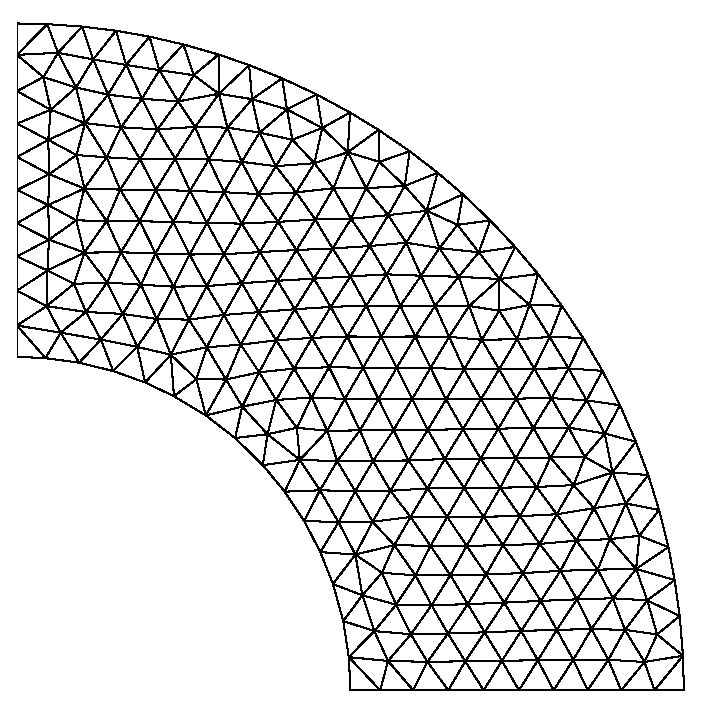
\includegraphics[width=0.4\textwidth]{mesh.eps}
  \caption{Mesh of upper right region of the annulus}
  \label{fig:MSH_ANN}
\end{figure}

\index{init\_Mesh@{\tt init\_Mesh}|)}


\section{Loading, Saving and Plotting Meshes}
\label{sect:IO}

\subsection{Loading and Saving Meshes} \index{mesh!loading} \index{mesh!saving} \label{ssect:load_save_mesh}

\LIBNAME offers the possibility to load and save basic meshes, containing the fields {\tt Coordinates} and {\tt Elements},
from and to files in ASCII format. Loading and saving a mesh from or to the files {\tt Coordinates.dat} and
{\tt Elements.dat} can be done by the the following two lines of code \\

\noindent {\tt >> Mesh = \ttitindex{load\_Mesh}('Coordinates.dat','Elements.dat');} \\
{\tt >> \ttitindex{save\_Mesh}(Mesh,'Coordinates.dat','Elements.dat');} \\

\subsection{Plotting Routines} \index{plot!mesh|(} \index{mesh!plotting|(} \label{ssect:plot_mesh}

 In the current version there are three different types of mesh plotting routines implemented -- \ttindex{plot\_Mesh}, \ttindex{plot\_Qual} and \ttindex{plot\_USR}. Besides, \ttindex{plot\_DomBd} plots the boundary of a mesh. All plotting routines are stored in the folder {\tt /Lib/Plots} and explained in the following. 

\subsubsection{Plot of Elements}

 The first plotting routine prints out the elements of a mesh. %% new: by Annegret Burtscher -->
 It is called by one of the following lines: \\

\noindent {\tt >> H = \ttitindex{plot\_Mesh}(Mesh);} \\

 For an example see figure \ref{fig:MSH_ANN}. It is also possible to add specific element, edge and vertex labels to a plot by specifying an optional string argument: \\

 \noindent {\tt >> H = plot\_Mesh(Mesh,Opt);} \\
 
 Here {\tt Opt} is a character string made from one element from any (or all) of the characters described in table \ref{tab:plot_mesh_opt}.

\begin{table}[htb]
  \centering
  \begin{tabular}{p{0.5cm}p{8.5cm}}
	{\tt 'f'} & {\small does not create a new window for the mesh plot} \\
	{\tt 'p'} & {\small adds vertex labels to the plot using {\tt add\_VertLabels}} \\
	{\tt 't'} & {\small adds element labels/flats to the plot using {\tt add\_ElemLabels}} \\
	{\tt 'e'} & {\small adds edge labels/flags to the plot using {\tt add\_EdgeLabels}} \\
	{\tt 'a'} & {\small displays axes on the plot} \\
	{\tt 's'} & {\small adds title and axes labels to the plot}
  \end{tabular}
  \caption{Optional characters {\tt Opt}}
  \label{tab:plot_mesh_opt}
\end{table}

 The following already mentioned subfunctions are used:
\begin{itemize}
	\item \ttitindex{add\_VertLabels} adds vertex labels to the current figure and is called by

		\noindent {\tt >> add\_VertLabels(Coordinates);}

	\item \ttitindex{add\_ElemLabels} adds the element labels {\tt Labels} to the current figure by

		\noindent {\tt >> add\_ElemLabels(Coordinates,Elements,Labels);}

	\item \ttitindex{add\_EdgeLabels} adds the edge labels {\tt Labels} to the current figure by

		\noindent {\tt >> add\_EdgeLabels(Coordinates,Edges,Labels);} \\

\end{itemize} %% <-- new: by Annegret Burtscher


\subsubsection{Element Quality Plot} \index{plot!element quality}

 The plotting routine of the second type generates a 2D plot of the element quality for all triangles $T$ contained in the mesh according to the formula
\begin{eqnarray}
\label{eq:ELEM_QUAL}
  q(T) = 2\frac{r_{\operatorname{in}}}{r_{\operatorname{out}}}
\end{eqnarray}
where $r_{\operatorname{out}}$ is the radius of the circumscribed circle and $r_{\operatorname{in}}$ of the inscribed
circle. %% new: by Annegret Burtscher -->
It is called by \\

\noindent {\tt >> H = \ttitindex{plot\_Qual}(Mesh);} \\

\noindent and returns the handle {\tt H} to the figure. %% <-- new: by Annegret Burtscher 
For an example see figure \ref{fig:ELEM_QUAL}.

\begin{figure}[htb]
  \centering
  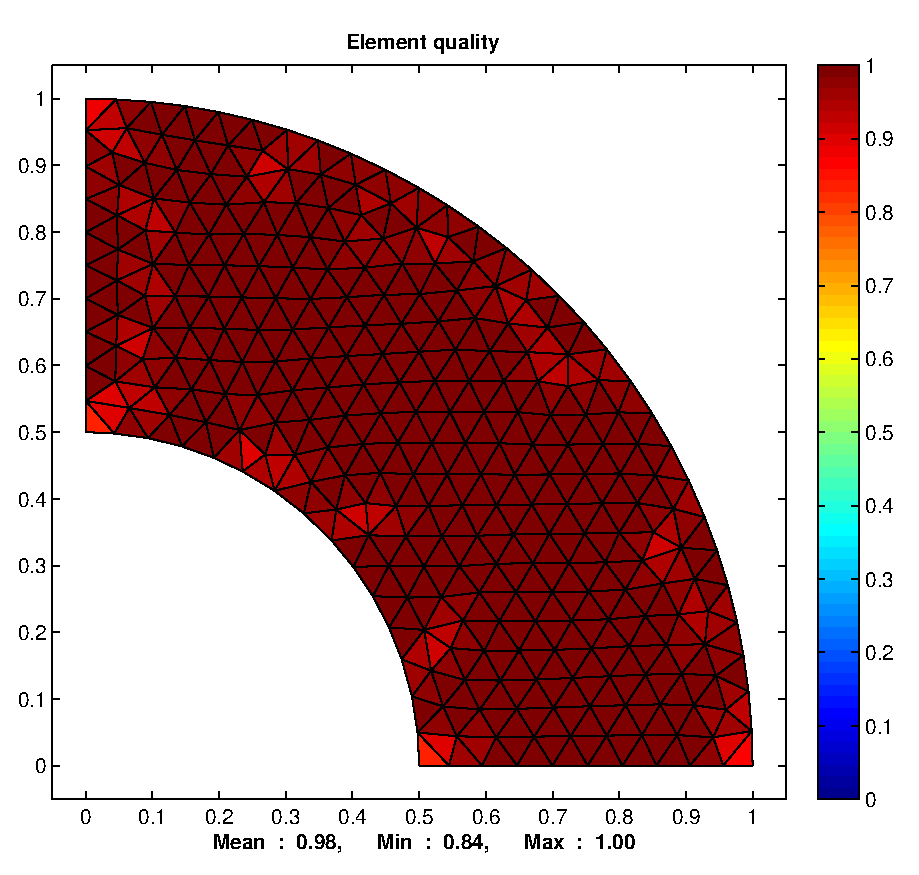
\includegraphics[width=0.5\textwidth]{qual.eps}
  \caption{Element quality plot}
  \label{fig:ELEM_QUAL}
\end{figure}


\subsubsection{Plot of Uniform Similarity Region} \index{plot!university similarity region}
 
 The plotting routine of the third kind generates plot of the uniform similarity region for triangles as described in the review article by D. A. Field \cite{FIE00}. The uniform similarity region seperates all elements into {\em obtuse} triangles with one angle larger than $\pi/2$ , and {\em acute} triangles. The elements above the half circle are acute, whereas the elements below are obtuse. %% new: by Annegret Burtscher -->
The function \ttitindex{plot\_USR} is called by \\

\noindent {\tt >> H = plot\_USR(Mesh);} \\ %% <-- new: by Annegret Burtscher

 For an example of this plot see figure \ref{fig:USR}.

\begin{figure}[htb]
  \centering
  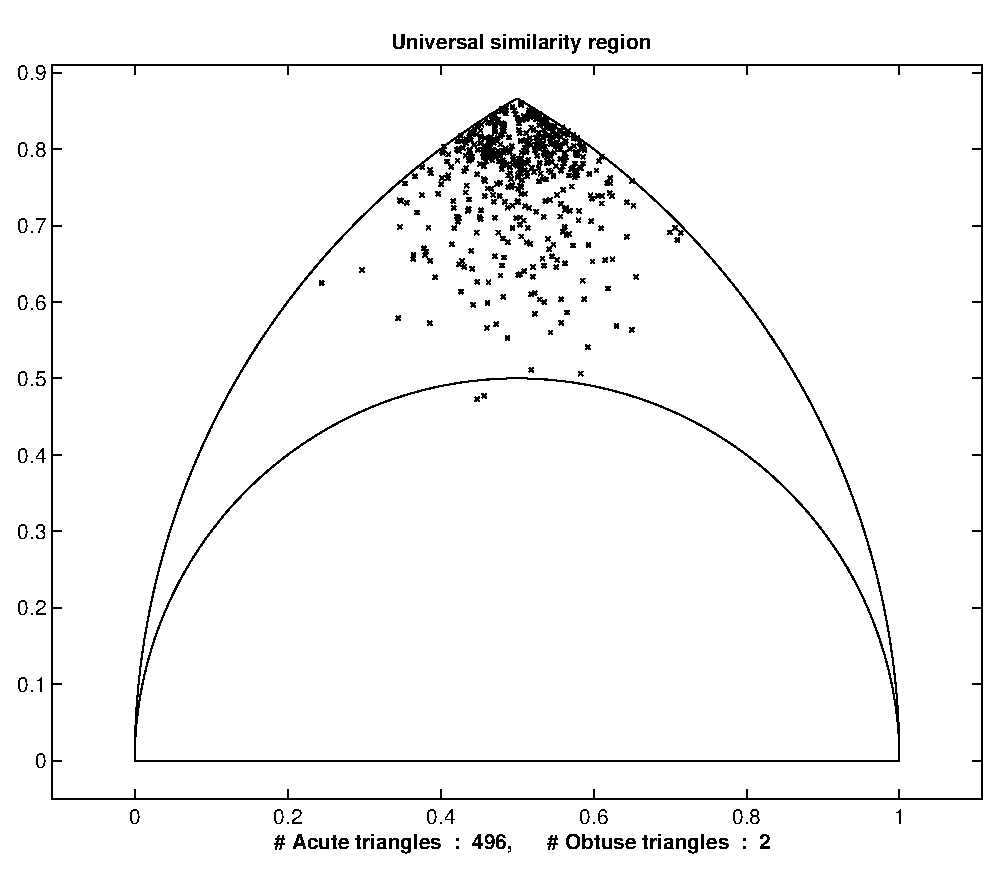
\includegraphics[width=0.5\textwidth]{usr.eps}
  \caption{Plot of the uniform similarity region}
  \label{fig:USR}
\end{figure}

\index{mesh!plotting|)}
\index{plot!mesh|)}

%% new: by Annegret Burtscher -->
\subsubsection{Boundary Plot} \index{plot!mesh boundary|(}

 Additionally, the function \ttitindex{plot\_DomBd} generates a 2D boundary plot of the mesh boundary. The string characters {\tt 'a'} and {\tt 's'} may be added in the argument {\tt Opt}, see table \ref{tab:plot_mesh_opt}. Therefore it is called by one of the following lines: \\

\noindent {\tt >> H = plot\_DomBd(Mesh);} \\
\noindent {\tt >> H = plot\_DomBd(Mesh,Opt);} \\

 with e.g. {\tt Opt = 'as'}.
%% <-- new: by Annegret Burtscher


\section{Mesh Refinements} \index{mesh!refinements}
\label{sect:MR}

 In order to obtain accurate numerical approximate solutions to partial differential equations it is necessary to refine meshes up to a very high degree. The current version of \LIBNAME supports uniform red refinements and adaptive green refinenments of the mesh.


\subsection{Uniform Mesh Refinements}
\label{sect:UMR}

 Uniform mesh refinement is based on the idea to subdivide every element of the mesh into four elements. For triangles this refinement strategy can be seen in figure \ref{fig:REG}.

\begin{figure}[htb]
  \centering
  \begin{minipage}[c]{0.8\textwidth}
    \includegraphics[width=0.4\textwidth]{REG_org.eps} \hfill
    \includegraphics[width=0.4\textwidth]{REG_ref.eps}
  \end{minipage}
  \caption{Red refinement for triangular elements}
  \label{fig:REG}
\end{figure}

In order to be able to perform regular red refinement steps, the mesh data structure needs to provide additional information
about the edges forming part of the boundary and interior edges of the domain. This additional information is contained in
the field {\tt BdFlags} of the mesh. This array can be used to parametrize parts of the boundary of the domain. In the current
version of \LIBNAME we use the convention, that {\em edges forming part of the boundary have negative boundary flags}. For further
details concerning the mesh data structure used for uniform red refinements consider table \ref{tab:MSH_R}.

\begin{table}[htb]
  \begin{tabular}{p{2cm}p{9cm}}
    {\tt Coordinates} & {\small $M$-by-$2$ matrix specifying all vertex coordinates}                \\
    {\tt Elements}    & {\small $N$-by-$3$ or $N$-by-$4$ matrix connecting vertices into elements}  \\
    {\tt Edges}       & {\small $P$-by-$2$ matrix specifying all edges of the mesh}                 \\
    \ttitindex{BdFlags}     & {\small $P$-by-$1$ matrix specofying the the boundary flags
                        each edge in the mesh. If edge number {\tt i} belongs to the
                        boundary, then {\tt BdFlags(i)} must be smaller than zero.
                        Boundary flags can be used to parametrize parts of the boundary}            \\
    {\tt Vert2Edge}   & {\small $M$-by-$M$ sparse matrix specifying the edge number
                        of the edge connecting vertices {\tt i} and {\tt j} (or zero
                        if there is no edge)}
  \end{tabular}
  \caption{Mesh data structure for uniform red refinements}
  \label{tab:MSH_R}
\end{table}

To perform one uniform red refinement step with a mesh suitable for red refinements just type the following line
into the \MATLAB command window \\

\noindent{\tt >> Mesh = \ttitindex{refine\_REG}(Mesh);} \\ \label{refine_REG}

 \noindent During the refinement procedure it is also possible to project the new vertices created on the boundary edges of the mesh onto the boundary of the domain. This is necessary if the boundary can not be resembled exactly using triangles, e.g. circles. To do so just type the following command into the \MATLAB command window \\

\noindent{\tt >> Mesh = refine\_REG(Mesh,DHandle,DParam);} \\

 \noindent here {\tt DHandle} denotes a \MATLAB function handle or inline object to a signed distance function specifying the geometry of the domain, as described in section \ref{sect:MGEN}. This distance function is used to move new vertices generated on boundary edges towards the boundary of the domain. {\tt DParam} denotes an optional variable length argument list which is directly handled to the distance function.

 Furthermore it is possible to extend a fine mesh, which has been obtained by one uniform red refinement from a coarse mesh, with multilevel data, that specifies the locations of vertices, elements and edges of the fine mesh on the coarse mesh. For details concerning these additional fields please consider table \ref{tab:MLEVEL}.

\begin{table}[htb]
  \begin{tabular}{p{2cm}p{9cm}}
    {\tt Father\_Vert} & \small $M$-by-$3$ matrix specifying the ancestor vertex/edge/element of each vertex
                         in the current mesh. If vertex {\tt i} is located on a vertex of the coarse mesh,
                         then {\tt Father\_Vert(i,1)} points to that father vertex in the coarse mesh.
                         If vertex {\tt i} is located on an edge of the coarse mesh, then {\tt Father\_Vert(i,2)}
                         points to that edge in the coarse mesh. Last bu not least, if vertex {\tt i} is located
                         on an element of the coarse mesh, then {\tt Father\_Vert(i,3)} points to that element.     \\
    {\tt Father\_Elem} & \small $N$-by-$1$ matrix specifying the ancestor element of each element in the current
                         mesh. {\tt Father\_Elem(i)} points to the father element of element {\tt i} in the coarse
                         mesh.                                                                                         \\
    {\tt Father\_Edge} & \small $P$-by-$2$ matrix specifying the ancestor edge/element of each edge in the
                         current mesh. If edge {\tt i} is located inside an element of the coarse mesh, then
                         {\tt Father\_Edge(i,2)} points to that element in the coarse mesh, else
                         {\tt Father\_Edge(i,1)} points to the father edge of edge {\tt i} in the coarse mesh.
  \end{tabular}
  \caption{Additional multilevel data fields}
  \label{tab:MLEVEL}
\end{table}

 {\noindent} In order to append these additional fields to a refined mesh just simply type in the following command into the \MATLAB command window \\

\noindent {\tt >> Mesh = \ttitindex{add\_MLevel}(Mesh);} \\

 \noindent No information about the coarse mesh is needed, since it is possible to deduce all vital information from the refinement algorithm.


\subsection{Adaptive Mesh Refinements}
\label{sect:AMR}

 The current version of \LIBNAME also supports adaptive mesh refinement from an initial coarse mesh. Up to now \LIBNAME only supports the largest edge bisection algorithm for triangular elements.

 Adaptive mesh refinements are based on a-posteriori error estimates. Error estimates for every element can be computed and then the elements where the imposed error is large are marked for a refinement. The largest edge bisection algorithm is one way to subdivide triangles.

 The implementation of the largest edge bisection is based on the data structure and algorithms presented in the manual of the adaptive hierarchical finite element toolbox ALBERT of A. Schmidt and K.G. Siebert \cite{ALB00}. For every element one of its edges is marked as the refinement edge, and the element into two elements by cutting this edge at its midpoint (green refinement).

 In our implementation we use the largest edge bisection in Mitchell's notation \cite{MI89}, which relies on the convention that the local enumeration of vertices in all elements is given in such a way that the longest edge is located between local vertex $1$ and $2$. Now for every element the longest edge is marked as the refinement edge and for all child elements the newly created vertex at the midpoint of this edge obtains the highest local vertex number. For details on the local element enumeration and the splitting process se figure \ref{fig:LEB}.

 Sometimes the refinement edge of a neighbour does not coincide with the refinement edge of the current element. Such a neighbour is not compatibly divisible and a green refinement on the current element would create a hanging node. Thus we have to perform a green refinement at the neighbours refinement edge first. The child of such a neighbour at the common edge is then compatibly divisible. Thus it can happen that elements not marked for refinement will be refined during the refinement procedure.

\begin{figure}[htb]
  \centering
  \begin{minipage}[c]{0.7\textwidth}
    \includegraphics[width=0.4\textwidth]{LEB_org.eps} \hfill
    \includegraphics[width=0.4\textwidth]{LEB_ref.eps}
  \end{minipage}
  \caption{largest edge bisection}
  \label{fig:LEB}
\end{figure}

 If an element is marked for green refinement we need to access the neighbouring element at the refinement edge and check wheter its local vertex enumeration is compatibly divisible with the current marked element. Thus for every element the data structure needs to provide us with a list of all the neighbouring elements, which is given by the field {\tt Neigh}, and the local enumeration of vertices for all neighbouring elements, which is given by the list {\tt Opp\_Vert}. For details see table \ref{tab:MSH_LEB}. This additional information can be created very easily by the following function call \\

\noindent{\tt >> Mesh = init\_LEB\index{init\_LEB@{\tt init\_LEB}}(Mesh);} \\

 \noindent which initializes the struct {\tt Mesh}, that contains the fields {\tt Coordinates}, {\tt Elements}, {\tt Edges}, {\tt BdFlags} and {\tt Vert2Edge} for largest edge bisection. For details on the mesh data structure needed see table \ref{tab:MSH_R} again.

\begin{table}[htb]
  \begin{tabular}{p{2cm}p{9cm}}
    {\tt Coordinates} & \small $M$-by-$2$ matrix specifying all vertex coordinates            \\
    {\tt Elements}    & \small $N$-by-$3$ matrix connecting the vertices into elements        \\
    {\tt Neigh}       & \small $N$-by-$3$ matrix specifying all elements sharing an edge
                        with the current element. For element {\tt i} {\tt Neigh(i,j)}
                        specifies the neighbouring element at the edge opposite of
                        vertex {\tt j}                                                        \\
    {\tt Opp\_Vert}   & \small $N$-by-$3$ matrix specifying the opposite local vertex of all
                        neighbours of an element. For element{\tt i} {\tt Neigh(i,j)}
                        specifies the local index of the opposite vertex of the
                        neighbouring element at the edge opposite of vertex {\tt j}
  \end{tabular}
  \caption{Data structure used for largest edge bisection}
  \label{tab:MSH_LEB}
\end{table}

 By using a-posteriori estimates a list of elements to be refined can be created by storing the corresponding labels in {\tt Marked\_Elements}. With this information and the struct {\tt Mesh} the following routine computes the refined mesh\\

\noindent{\tt >> Mesh = refine\_LEB\index{refine\_LEB@{\tt refine\_LEB}}(Mesh,Marked\_Elements);} \\

\section{Postprocessing} \index{mesh!postprocessing}

 In the current version of \LIBNAME a small amount of postprocessing routines are available.

\subsection{Mesh Translation, Rotation and Stretching}

 In order to translate a mesh by a vector {\tt x\_0}, or rotate a mesh by the angle {\tt phi} in counter-clockwise direction or stretch it by {\tt x\_dir} in $x$-direction and {\tt y\_dir} in $y$-direction just simply type the following commands into the \MATLAB command window \\

\noindent{\tt >> Mesh = shift\index{shift@{\tt shift}}(Mesh,x\_0);} \\
\noindent{\tt >> Mesh = rotate\index{rotate@{\tt rotate}}(Mesh,phi);} \\
\noindent{\tt >> Mesh = stretch\index{stretch@{\tt stretch}}(Mesh,x\_dir,y\_dir);} \\

\subsection{Laplacian Smoothing and Jiggle}

 The current version of \LIBNAME supports unconstrained Laplacian smoothing for triangular and quadrilateral elements. In order to prevent the domain from shrinking it is possible to fix positions of certain vertices of the mesh. In order to use the unconstrained Laplacian smoother simply type the following command into the \MATLAB command window \\

\noindent{\tt >> Mesh = smooth\index{smooth@{\tt smooth}}(Mesh,FixedPos);} \\

\noindent here {\tt FixedPos} is a $M$-by-$1$ matrix whose non-zero entries denote fixed vertices of the mesh. \index{mesh|)}

To make a mesh less uniform there is a function that randomly moves inner vertices. This can for example be useful to investigate convergence rates on more random grids. To call the function type

\noindent \texttt{>> Mesh = jiggle(Mesh,FixedPos);}

\noindent Usually there is a jiggle parameter specified and based on which the Mesh is processed. The typical code segment can be found below.

\begin{lstlisting}
switch(JIG)
   case 1
     New_Mesh = Mesh;      
   case 2
     Loc = get_BdEdges(Mesh);
     Loc = unique([Mesh.Edges(Loc,1); Mesh.Edges(Loc,2)]);
     FixedPos = zeros(size(Mesh.Coordinates,1),1);
     FixedPos(Loc) = 1;
     New_Mesh = jiggle(Mesh,FixedPos);   
   case 3
     Loc = get_BdEdges(Mesh);
     Loc = unique([Mesh.Edges(Loc,1); Mesh.Edges(Loc,2)]);
     FixedPos = zeros(size(Mesh.Coordinates,1),1);
     FixedPos(Loc) = 1;
     New_Mesh = smooth(Mesh,FixedPos);
end
\end{lstlisting}



